%%%%%%%%%%%%%%%%%%%%%%%%%%%%%%%%%%%%%%%%%%%%%%%%%%%%%%%%%%%%%%%%%%%%%%%%
%                                                                      %
%     File: Thesis_Appendix_A.tex                                      %
%     Tex Master: Thesis.tex                                           %
%                                                                      %
%     Author: Andre C. Marta                                           %
%     Last modified :  2 Jul 2015                                      %
%                                                                      %
%%%%%%%%%%%%%%%%%%%%%%%%%%%%%%%%%%%%%%%%%%%%%%%%%%%%%%%%%%%%%%%%%%%%%%%%

\chapter{Supervised Learning}

Supervised Learning is the task of learning by example and it is divided into a training phase and a testing phase. In the first, the learner receives labelled data as input and the output is calculated, then based on a cost function that relates the predicted value with the actual value, the parameters of the model are updated such that the cost function is minimized. Then, in the second phase, the model is tested with new data, that it has never seen before, and its performance is evaluated. 
Supervised Learning can be divided into two groups: Classification and Regression. In classification, each item is assigned with a class or category, e.g. if an email is considered spam or not-spam, represents a binary classification problem. Whereas in regression, each item is assigned with a real-valued label. \cite{HanDataMining}
\\

In accordance with Kamei et al. \cite{kameiJIT} and Yang et al. \cite{yangJIT}, the typical predictive model used is the Logistic Regression. Here, other models are explored, such as Decision Trees and Artificial Neural Networks.

\section{Decision Trees}

Another potential candidate to treat our data may be a Decision Tree Classifier, which is categorized by having a flowchart-like tree structure, where there are nodes and branches. Each internal node denotes a test on an attribute and the branch represents the outcome of that test, then the nodes at the bottom of the tree, called \textit{leaf-nodes} whereas the topmost node is the \textit{root-node}, holds a class label. An example of such tree can be seen below\cite{HanDataMining}:

\begin{figure}[H]
	\centering
	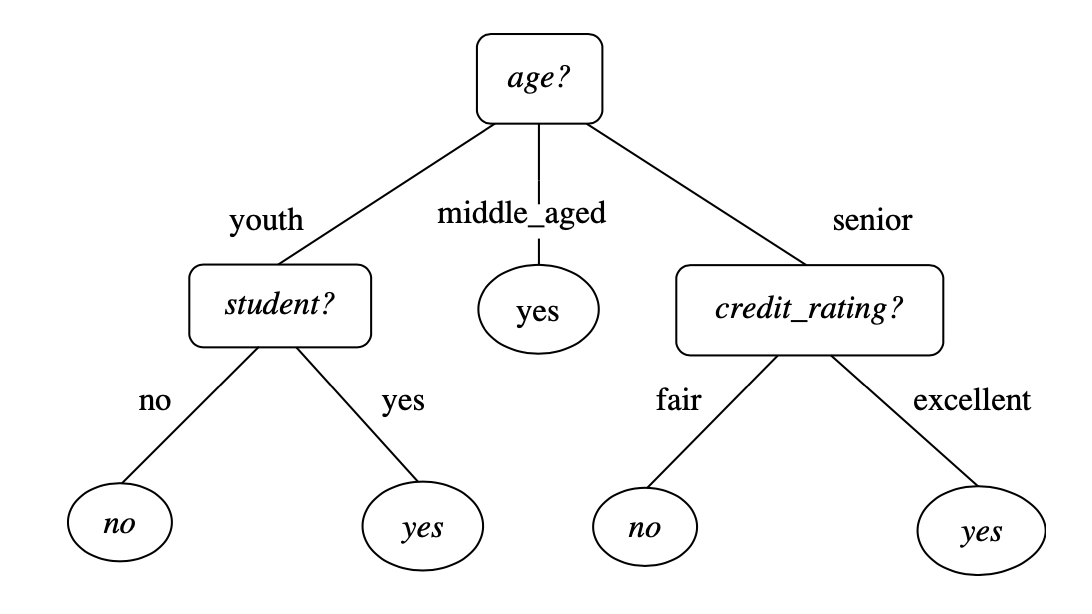
\includegraphics[scale=0.5, width=0.6\linewidth]{figures/DecisionTreeDiagram.png}
	\caption{Each internal (non-leaf) node represents a test on an attribute. Each leaf node represents a class (if the client is likely to buy the product yes/no )}
	\label{DTDiagram}
\end{figure} 

Then after training, when a new element serves as input of a Decision Tree, a path is traced from the root until the leaf node, revealing the prediction of which class that element belongs. Decision tree learning can be based in several algorithms. The most commonly used are ID3 ( Iterative Dichotomiser 3) , C4.5 and CART (Classification and Regression Trees). In this work, the chosen algorithm is provided by the \textit{scikit-learn} package and it uses an optimized version of CART. The mathematical formulation is as follows: 

\subsection{Mathematical formulation}

Given training vectors $x_i \in \Re^n, i = {1 , ... m} $ and a class label vector $y \in \Re^m$, a decision tree recursively partitions the space such that the samples equally labeled are grouped together. 

Considering the data at node $l$ be represented by $D$. For each candidate split $Q= (j, t_l),$, where $j$ corresponds to the \textit{j-th} feature and $t_m$ the threshold, partition the data into the subsets $D_{left}(\theta)$ and $D_{rigth}(\theta) $.

\begin{align}
	D_{left}(\theta) &= (x,y) | x_j \le t_l \\
	D_{right}(\theta) &= D \ D_{left}
\end{align}

Then, because data is not easily separable,i.e. partitions not often contain elements with the same class label, one defines a criterion called \textit{impurity}, that measures the probability of finding a mislabelled element in the subset. The impurity at $m$ is determined by using an impurity function $H()$, that depends if the task is classification or regression. 

\begin{equation}
	G(D,\theta) = \frac{n_{left}}{N_l}H(G(D_{left},\theta)) + \frac{n_{right}}{N_l}H(G(D_{right},\theta)) 
\end{equation}

where $n_{left}$ is the number of attributes partitioned to the left, $n_{right}$ to the right and $N_m$ the total number of attributes in a node. The function H() is commonly defined \\

as Gini Impurity: 
\begin{equation}
	H(D_m) = \sum_k p_{mk}(1-p_{mk})
\end{equation}

as Entropy:
\begin{equation}
	H(D_m) = -\sum_k p_{mk}(log(p_{mk})
\end{equation}

where $p_{mk}$ is the probability that an item $k$ with label $m$ is chosen.

The goal is to select parameters such that the impurity is minimised, such that:

\begin{equation}
	\theta^* = argmin_{\theta}  G(D, \theta)
\end{equation} 

Finally, recursively apply the same reasoning to subsets $D_{left}(\theta^*)$ and $D_{right}(\theta^*)$, until maximum tree depth reached, i.e. $N_m < min_{samples}$ \cite{DTform}


\section{Artificial Neural Networks}

In general terms, a neural network (NN) is a set of connected input/output units in which each connection has a weight associated with it. The weights are adjusted during the learning phase to help the network predict the correct class label of the input vectors.
\\

In light of the knowledge psychologists and neurobiologist have on the structure of the human brain, more precisely on how neurons pass information to one another, this way it was possible to look for methods to develop and test computational analogues of neurons. Generally, a NN is defined as a set of input/output \textit{units} (or \textit{perceptrons}) that are connected. Each connection has a weight associated with it, and these weights are adjusted in such manner, that the network is able to correctly predict the class label of the input data. The most popular algorithm for NN learning is \textit{back-propagation}, which gained popularity since 1980. \cite{HanDataMining}
\\

Usually, NN training phase involves a long period of time and a several number of parameters have to be set to build the network's structure and architecture. However, there is no formal rule to determine their optimality and this is achieved empirically, by running different experiments. This, nonetheless, raises an issue of poor interpretability, that makes it hard for humans to grasp what the optimal parameters mean. 
On the other hand, NN's compensate on easy-going implementation and ability to deal with noisy data and, so far, have been used to solve many real-world problems, such as hand written text recognition, medical diagnosis and finance \cite{HanDataMining}.
\\

In the following sections, the reader is guided in detail through the architecture of a NN and given a brief explanation of how back-propagation works.

\subsection{Perceptron}

A perceptron is the most elementary unit of a NN. In similarity to brain cells, that are composed by dendrites, that receive electric signals (input), the nucleus that processes them and the axon, that sends too an electric signal to other neurons (output). In our case, the perceptron receives a vector of inputs ${x_1, x_2,... x_n}$ and associated to each one there are weights ${w_1,w_2,...w_n}$ that symbolize the influence each input has on the output. As an example, consider a perceptron with an input vector composed of 3 inputs ${x_1, x_2, x_3}$.

\begin{figure}[H]
	\centering
	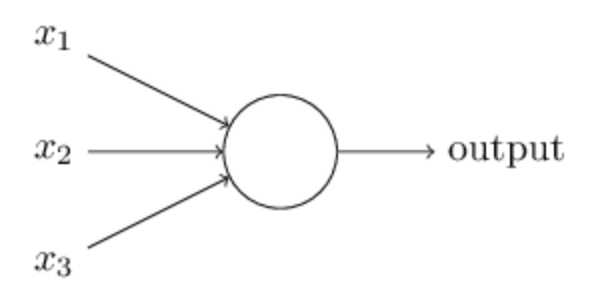
\includegraphics[scale=0.5, width=0.35\linewidth]{figures/perceptron.png}
	\caption{Perceptron simple example)}
	\label{perceptron}
\end{figure} 

Let us say the desired output is either $0$ or $1$. This value shall be determined by weighing the sum $ \sum_j w_j x_j$ and checking if the value surpasses a given threshold \cite{nielsenneural}. So the output can be defined as: 

\begin{equation}
	\mbox{\textbf{output}} = \begin{cases} 0, & \mbox{if } \sum_j w_j x_j \le \mbox{ threshold} \\ 1, & \mbox{if } \sum_j w_j x_j > \mbox{ threshold} \end{cases}
\end{equation}

Also, one can replace $ \sum_j w_j x_j$ as the dot product $w \cdot x $ and move threshold to the other side of the equation and call it $b$, for bias.

\begin{equation}
	\mbox{\textbf{output}} = \begin{cases} 0, & \mbox{if } w \cdot x + b \le 0 \\ 1, & \mbox{if }  w \cdot x + b > 0 \end{cases}
\end{equation}

Here, the bias term can be thought as the susceptibility of the neuron being activated, the large the value of $b$, more easily the output is 1. 

\subsection{Activation Functions}
There is a problem related to the sensitivity the perceptron has when $w \cdot x + b $ is close to zero. Small changes in the weights may cause a drastic effect on the outcome, because the expression corresponds to a step function. What can be done is define an activation function $\sigma(z)$ that transforms the expression above. Commonly,  $\sigma(z)$ is defined as the sigmoid function $\sigma(z) = \frac{1}{1+e^{-z}}$ , or the rectifier function $\sigma(z) = max(0,z) $, comparing the three curves for the same values of $w_i$ and $b_i$:

\begin{figure}[H]
	\centering
	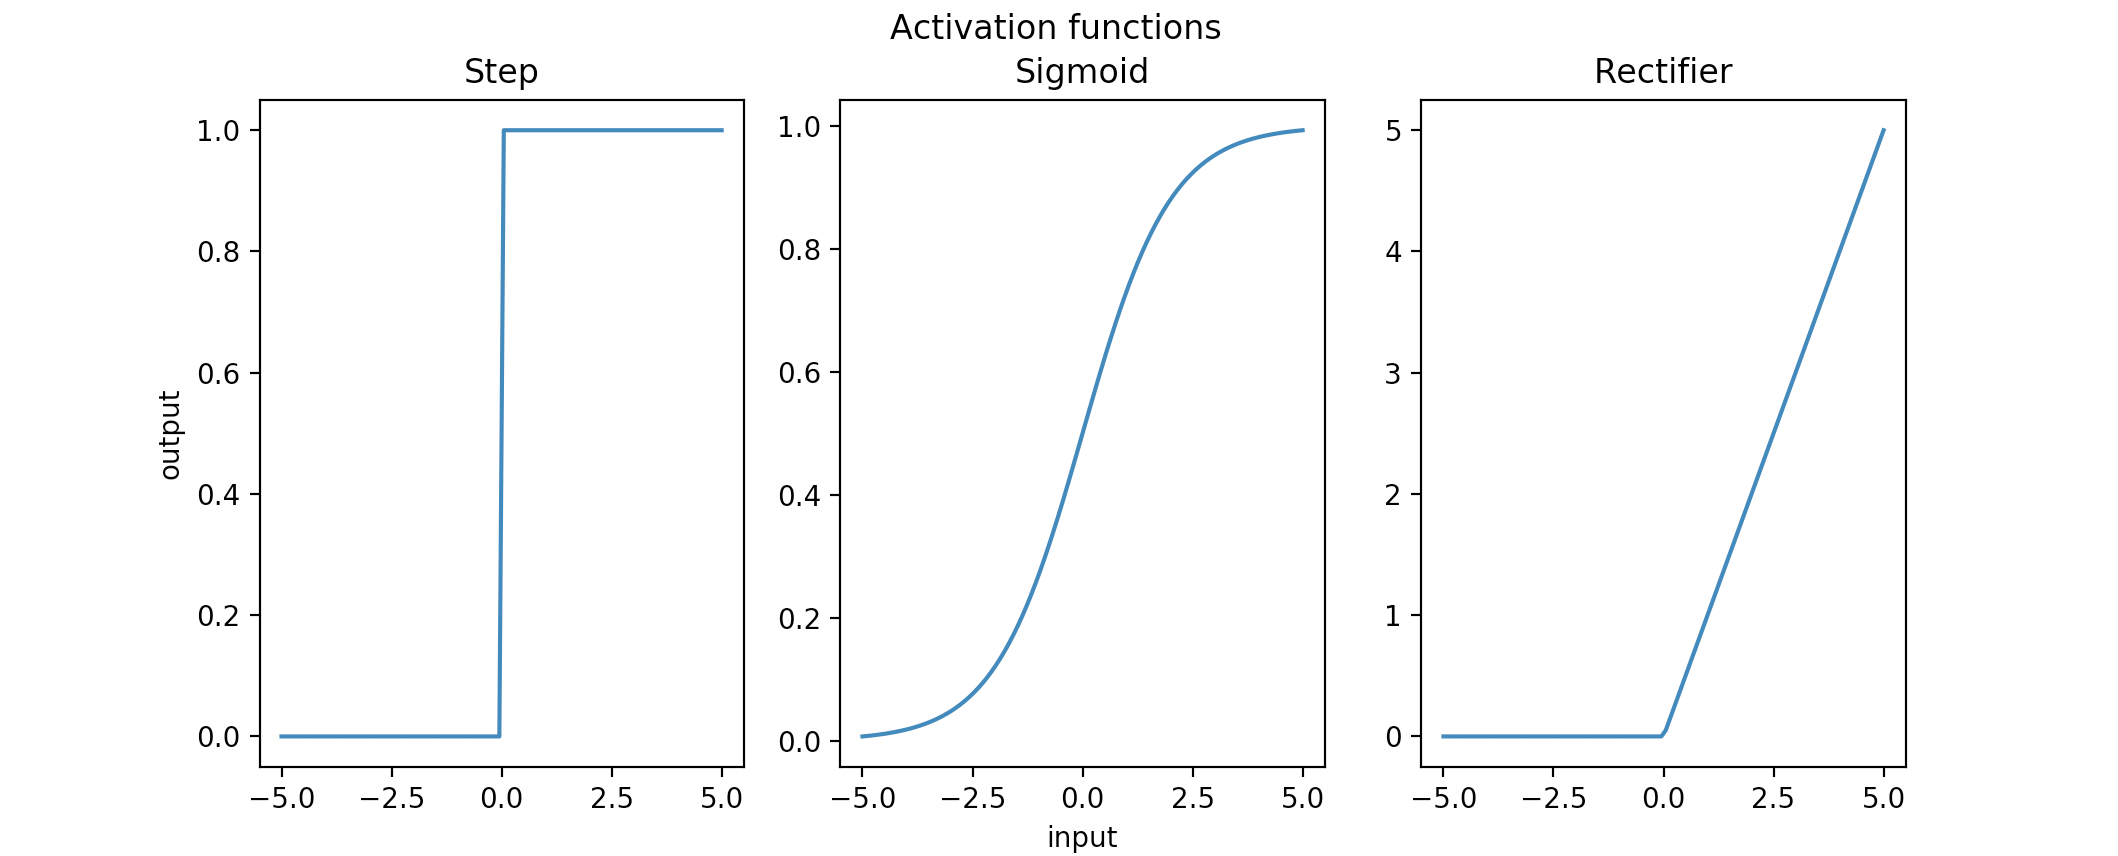
\includegraphics[scale=1, width=\linewidth]{figures/activationfunc.png}
	\caption{Comparative analysis of different activation functions (made in Python))}
	\label{activation}
\end{figure} 

In the first image, the transition from 0 to 1 is abrupt and steep, this way values that are close to the threshold can have dramatic distinctions in output and that is not desirable, because NN's learn by making little adjustments on the values of the weights. By using the sigmoid function values are smoothed out in a way that values no longer have a binary outcome, but rather a continuous and  progressive approximation to the values zero or one. For high positive inputs, the output is very close to one, the same happens for high negatives close to 0 (like in the step function case) and in between the curve is softer, also the sigmoid function in differentiable in all its domain. The third case corresponds to the rectifier function that only activates for positive values and due to its easy implementation, its usage because relevant in reaching high performance.

\subsection{NN architecture }

Now, very much alike the human brain, perceptrons are assembled together to form a connected structure called a network. By grouping perceptrons of the same type. - input, output or neither.- layers are form and there are three types: input layer, output layer and \textit{hidden} layer. The neuros that belong to the hidden layer are simply neither input nor output neurons, they serve as a mean of adding more complex relations between the variables input and weights. In terms of configuration, there is only one input layer and one output layer, with variable size. However multiple hidden layers may exist. Let us take the following example with an input vector of size $6$, an output vector with size $1$ and $2$ hidden layers of size $4$ and $3$. \cite{nielsenneural}.


\begin{figure}[H]
	\centering
	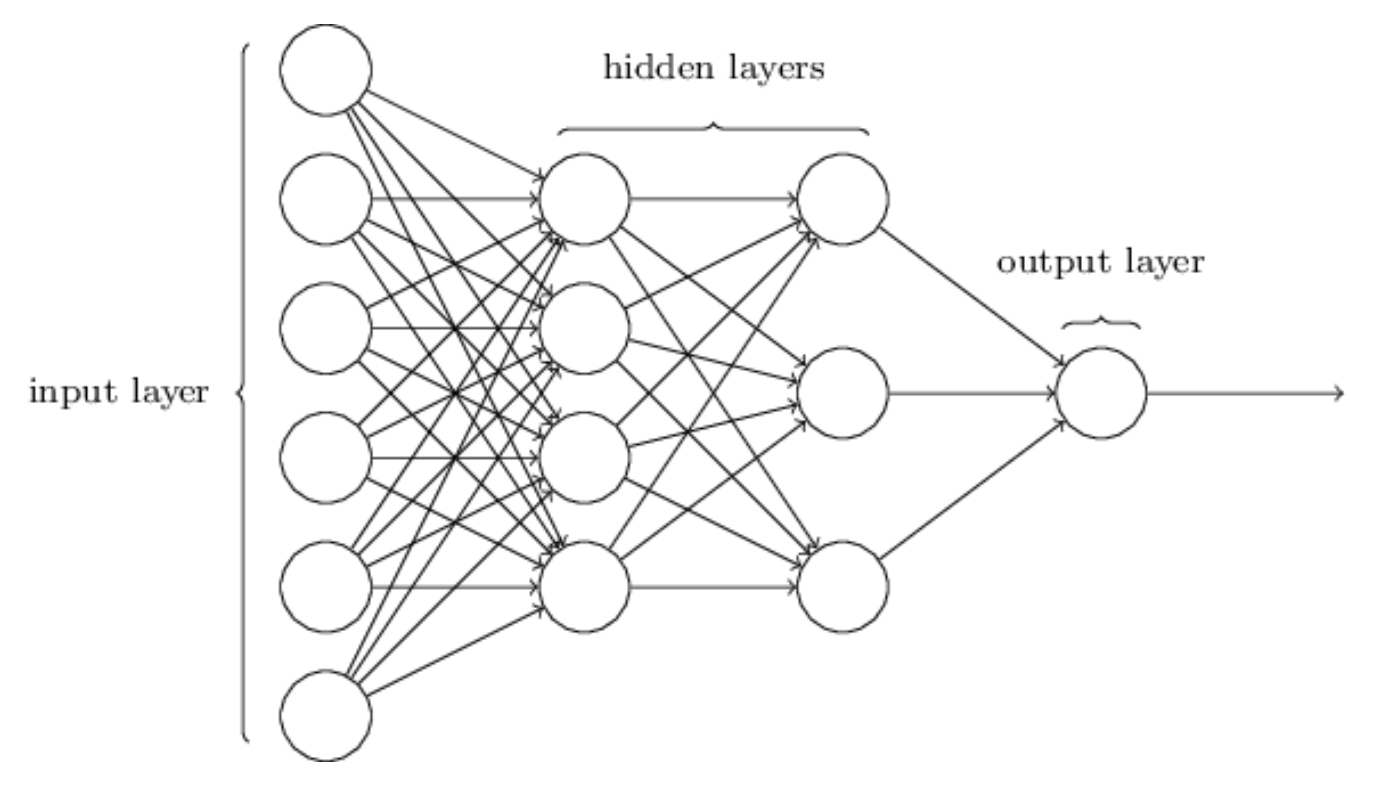
\includegraphics[scale=0.5, width=0.65\linewidth]{figures/nnarch.png}
	\caption{Architecture example of a NN \cite{nielsenneural}}
	\label{nnarch}
\end{figure} 

Every node as a connection to a node from the next layer, but what is changeable is the number of hidden layers and the number of nodes in each layer. Although there are some heuristics to determine the best configuration.- like choosing the number of neurons by averaging the number of neurons in the input and output layer.-  each dataset has its own characteristics, it becomes difficult to come up with a rule of thumb that works in generality, so one has to determine the parameters by running experiments.\cite{nielsenneural}
\\

To wrap up the functioning of a NN,  from an input vector $x$, the neurons from the next layer will be activated or not by computing $w \cdot x + b$, then the same process occurs until the output node is reached, in this case yielding the result $1$ or $0$, this left-to-right process is called \textit{forward-propagation}. Of course, this is not the process of learning, most likely if one compares the predicted result with the actual value, it is a $50 \%$ chance of being correct. So how does a NN learn?

\subsection{Learning with Gradient Descent}

As mentioned above, the desired result is achieved once the difference between the predicted value $\hat{y}$ and the actual actual $y$ is minimized. The goal is to find an algorithm that will indicate which values for weights and biases will produce the correct output. In order to quantify the performance achieved so far, let us define a cost function $C(Y,\theta)$,where in the  dataset $Y$, $\theta$ are the parameters, , $m$ the total number of samples in the dataset and $i$ its index.:

\begin{equation}
	C(Y,\theta) = \frac{1}{2m}\sum_{i=1}^{m}(\hat{y}^{(i)} - y^{(i)})^2
\end{equation}

In this formula, one sees that it is close to zero, exactly when the predicted value matches the expected value. A possible approach to reach this result could be to brute force the values of the parameters: trying out several combinations of weights and biases, narrowing down in each iteration, eventually converging towards the quadratic value, or the minimum of the cost function. However, this approach does not scale. With just $25$ weights and assuming each weight can have $1,000$ different values, there are $1000^{25} =10^{75}$ possible combinations, which is infeasible to compute, even for modern supercomputers\cite{ml_phys}.
\\

A more efficient strategy is to use Gradient Descent to minimize the cost function. The first step would be to randomly initialize all the weights and bias, similar to the initial condition of a differential equation, and then calculate the output $\hat{y}$ and compute the cost function. Most likely, it will not yield a result close to the minimum, so now one needs to know is what direction of the curve points towards the minimum and then "jump" a step towards that direction. This is achieved by calculating the gradient of the cost function, with respect to $\theta$.

\begin{align}
	v_t &= \eta_t \nabla_{\theta} C(Y,\theta) \\
	\theta_{t+1} &= 	\theta_{t}  - v_t
\end{align}

where  $\eta_t$ is the \textit{learning rate} that defines the length of the step taken in the direction of the gradient , at time step t. By configuring a small learning rate it is guaranteed local minimum convergence, however implying a high computational cost and not assuring an optimal solution by landing on a global minimum. On the other hand, by choosing a large learning rate the algorithm can become unstable and overshoot the minimum. (possible oscillatory dead-end).\cite{ml_phys}.  Minimising a cost function looks this:

\begin{figure}[H]
	\centering
	\begin{minipage}{.5\textwidth}
		\centering
		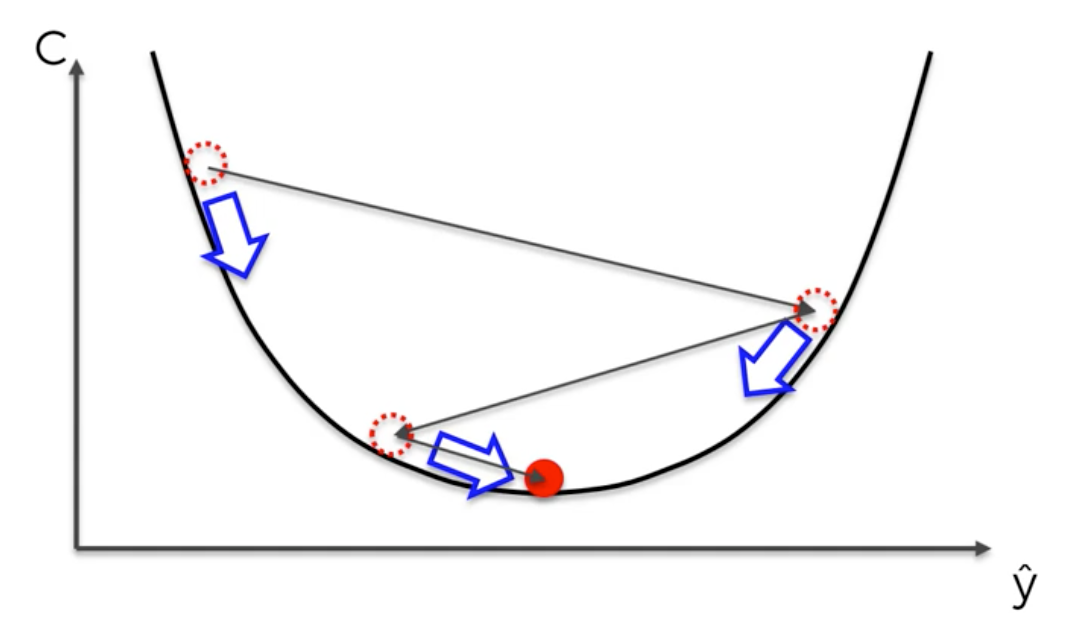
\includegraphics[width=.9\linewidth]{figures/graddesc.png}
		\label{fig:test1}
	\end{minipage}%
	\begin{minipage}{.5\textwidth}
		\centering
		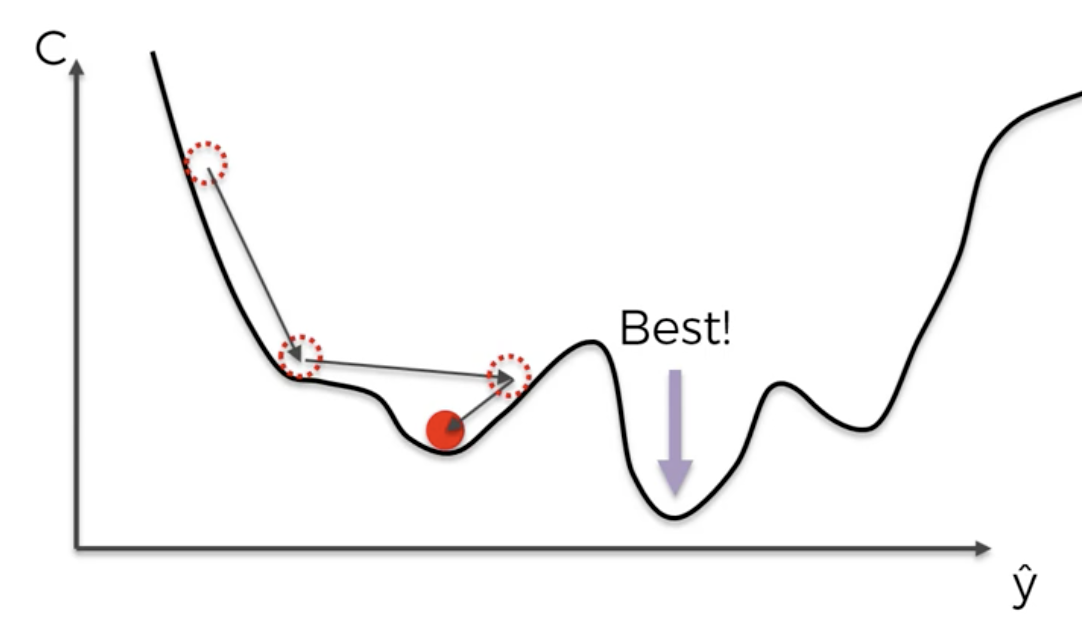
\includegraphics[width=.9\linewidth]{figures/graddesc2.png}
		\label{fig:test2}
	\end{minipage}
	\caption{Global and Local minimum determination \cite{udemyDS}}
\end{figure}

In this one dimensional example, the gradient yields the direction towards the minimum and the learning rate determines the length of the step. However, in the second case, there are some cases where convergence is sub-optimal. This information hints the conclusion that choosing simple gradient descent, as our minimizing algorithm, has many limitations, namely:

\begin{itemize}
	\item \textit{Finding global minimum} - only local minimum are guaranteed to be found under the gradient descent algorithm.
	\item \textit{Sensitive to initial conditions} - depending on the starting point, the final location most likely will be a different minimun, hence there is a high dependency on initial conditions.
	\item \textit{Sensitive to learning rate} - as seen above, learning rate can have a huge impact on the algorithm's convergence.
	\item \textit{Computationally expensive} - although better than brute force, when handling large datasets, computation rapidly increases cost. Possible solution is to just apply the algorithm to a subset or \textit{"mini-batch"}
	\item \textit{Isotropic parameter-space} - Learning rate is always the same independent of the "landscape". Ideally, the learning rate should be larger in flatter surfaces and smaller in steeper ones. \cite{ml_phys} 
\end{itemize}


\subsection{Stochastic Gradient Descent (SGD)}

To handle the limitations described in the section above, a novel, more efficient algorithm is proposed: the Stochastic Gradient Descent (SGD). The advantage is that, not only the method is more computationally efficient, but it also deals with non-convex cost-functions, on the contrary of simple gradient descent, also called \textit{batch} gradient descent method, because it plugs every item of the dataset into the neural network, obtains the predicted values, calculates the cost function by summing the square differences to the expected value and only then the weights are adjusted. \cite{nielsenneural}
SGD works in a different way, here the batch is divided into $n/M$ subsets or \textit{mini-batches} $B_k, k={1,...,n/M}$, where $n$ is the total number of data points and $M$ the mini-batch size. The gradient now takes the following form: 

\begin{equation}
	\nabla_{\theta} C(Y,\theta) = \frac{1}{2m}\sum_{i=1}^{n}\nabla_{\theta} (\hat{y}^{(i)} - y^{(i)})^2 \rightarrow \frac{1}{2m}\sum_{i \in B_k}\nabla_{\theta} (\hat{y}^{(i)} - y^{(i)})^2
\end{equation}


Each mini-batch $B_k$ is plugged into the NN, the cost function is calculated and the weights are updated. This process repeats $k$ times until the whole data set is covered. A full run over all $n$ points is denoted as an \textit{epoch}. \cite{ml_phys}
\\

In sum, SGD has two very important advantages: not only eliminates the local minimum convergence problem, by introducing stochasticity , but also it is much more efficient in computational power, because only a subset of $n$ data points has to be used to approximate the gradient.


\subsection{Backpropagation}

So far, a review of the basic structure and training of NN has been provided: starting from the elementary unit.- the perceptron - up to how many of them can be assembled, covering the most common types of activation functions. Then the concept of forward propagation was introduced along with a cost function that allows to judge whether the model created explains the observations. 
\\

The goal is to minimise the cost function, resorting, in a first approach, to the gradient descent method which, as seen above, has severe limitations, concluding that the Stochastic Gradient Descent algorithm is most suited for this task. However, SGD still requires us to calculate the derivative of the cost function with respect to every parameter of the NN. So a forward step has to be taken to compute these quantities efficiently. - via the \textbf{backpropagation} algorithm. - to avoid calculating as many derivatives as there are parameters. Also backpropagation enables the determination of the contribution of each weight and bias to the cost function, altering more, the weights and biases that contribute the most, thus understanding how changing these particular values will affect the overall behaviour. \cite{nielsenneural}
\\

The algorithm can be summarized into four equations, but first, let us define some notation. Assuming a network composed of $L$ layers with index $l = {1,... L}$ and denote by $w_{j,k}^l$ the weight connecting from the \textit{k-th} neuron of layer \textit{l-1} to the \textit{j-th} neuron in layer \textit{j}. The bias of this neuron is denoted $b_l^j$. By constructing, one can write the activation function $a_j^l$ of the  \textit{j-th} neuron in the  \textit{l-th} layer, by recursively writing the relation to the activation $a_j^{l-1}$ of neurons in the previous layer \textit{l-1}.

\begin{equation}
	a_j^l = \sigma\bigg(\sum_{k}\omega_{j,k}^l a_k^{l-1} + b_j^{l} \bigg) = \sigma(z_j^l)
	\label{first}
\end{equation}

When calculating the cost function $C$, one only needs to take directly into account the activation from the neurons of layer $L$, of course the influence of the neurons from previous layers is underlying. So one can define the quantity, $ \Delta_j^L$, which is the error of the \textit{i-th} neuron in layer L , as the change it will cause on the cost function $C$, regarding weighted input $z_j^L$:

\begin{equation}
	\Delta_j^L = \frac{\partial C}{\partial z_j^L}
\end{equation}

Generally, defining the error of neuron $j$ of any layer $l$ and applying the chain rule to obtain the first equation of the algorithm:

\begin{equation}
	\Delta_j^l = \frac{\partial C}{\partial z_j^l} =  \frac{\partial C}{\partial a_j^l} \frac{\partial a_j^l}{\partial z_j^l} =  \frac{\partial C}{\partial a_j^l} \sigma '(z_j^l)
	\label{backprop1}
\end{equation}

Now, one can relate the error function $ \Delta_j^L$ to the bias $b_j^{l}$ to obtain the second backpropagation relation:

\begin{equation}
	\Delta_j^L = \frac{\partial C}{\partial z_j^L} = \frac{\partial C}{\partial b_j^l} \frac{\partial b_j^l}{\partial z_j^l} = \frac{\partial C}{\partial b_j^l}
	\label{backprop2}
\end{equation}

Since, $\frac{\partial b_j^l}{\partial z_j^l} = 1$ , from \ref{first}. 
Furthermore to find another expression for the error, one can relate the neurons in layer $l$ with the neurons in layer $l+1$: 

\begin{align}
	\Delta_j^l &= \frac{\partial C}{\partial z_j^l} = \sum_k \frac{\partial C}{\partial z_k^{l+1}} \frac{\partial z_k^{l+1}}{\partial z_k^{l}} \\
	&= \sum_k  \Delta_k^{l+1}  \frac{\partial z_k^{l+1}}{\partial z_k^{l}} \\
	&= \bigg( \sum_k  \Delta_k^{l+1} \omega_{k,j}^{l+1}\bigg) \sigma '(z_j^l)
	\label{backprop3}
\end{align}


This is the third relation. Finally, to derive the final equation, one differentiates the cost function with respect to the weights $\omega_{j,k}^l:$

\begin{equation}
	\frac{\partial C}{\partial \omega_{j,k}^l} =\frac{\partial C}{\partial z_{j}^l}\frac{\partial z_{j}^l}{\partial \omega_{j,k}^l} = \Delta_j^{l} a_k^{l-1}
	\label{backprop4}
\end{equation}

The combination equations \ref{backprop1}, \ref{backprop2}, \ref{backprop3} and \ref{backprop4}, constitutes the backbone of the backpropagation algorithm that is used to train NN's in a very efficient way \cite{ml_phys}. It described in the following steps:
\\

\textbf{Backpropagation Algorithm:}
\begin{enumerate}
	\item \textbf{Activation at input layer} - compute the activations of the input layer $a_j^1$.
	\item \textbf{Forward propagation} - Through equation \ref{first}, determine the activations $a_j^1$ and the linear weigthed sum $z_j^l$, for each layer $l$.
	\item \textbf{Error at layer $L$} - calculate the error $\Delta_j^L $, using equation \ref{backprop2}.
	\item \textbf{Propagate the error "backwards"} - calculate the error $\Delta_j^l$, for all layers $l$, using equation \ref{backprop3}. 
	\item \textbf{Determine gradient} - use equation \ref{backprop2} and \ref{backprop4} to calculate  $\frac{\partial C}{\partial b_j^l}$ and $\frac{\partial C}{\partial \omega_{j,k}^l}$.
\end{enumerate}
\cite{ml_phys}

In sum, the application  of this algorithm consists on determining the error at the final layer and then "chain-ruling" our way back to the input layer,find out quickly how the cost function changes, when the weights and biases are altered. \cite{nielsenneural}


